\documentclass[12pt, a4paper]{article}

% ----- Packages -----
\usepackage[margin=1in]{geometry}
\usepackage{tikz}
\usetikzlibrary{arrows.meta, positioning, shapes.geometric}
\usepackage{amsmath}
\usepackage{xcolor}
\usepackage{parskip}

% ----- Styling -----
\definecolor{riseblue}{RGB}{0, 80, 158}
\newcommand{\moduleheader}[1]{
    \vspace{1cm}
    {\Large \textcolor{riseblue}{\textbf{#1}}}
    \vspace{0.3cm}
    \hrule
    \vspace{0.5cm}
}

\begin{document}

% ----- Title Page / Header -----
\begin{center}
    {\Huge \textbf{RISE Internship: Network Theory}} \\[0.3cm]
    {\Large \textit{Foundations \& Controllability Problem Set}} \\[0.5cm]
    \textbf{Mentor(s):} Danish \& \underline{\hspace{3cm}} \quad | \quad \textbf{Lab:} Dr. Mudassir Shabbir
\end{center}
\vspace{0.5cm}

% ----- Introduction -----
\section*{Introduction}
Welcome to the theoretical track of your research project! While we will be using Python and NetworkX to visualize massive datasets of social media networks, computer science research begins on paper. 

This document contains visual puzzles and mathematical exercises designed to test your intuition. At the end of each coding module, you will return to this sheet to complete the corresponding section. You do not need to write any code to solve these—just use logic, tracing, and the definitions you learned in the notebooks.

% ----- Module 1 -----
\moduleheader{Module 1: The Foundations}

\textbf{Problem 1.1: The Königsberg Rule (Nodes \& Connections)} \\
Below is a map of a fictional city consisting of four landmasses (Nodes A, B, C, and D) connected by bridges (Edges). In the notebook, you learned Euler's rule for the Königsberg puzzle: \textit{"If more than two nodes have an odd number of connections, crossing every bridge exactly once is impossible."}

\begin{center}
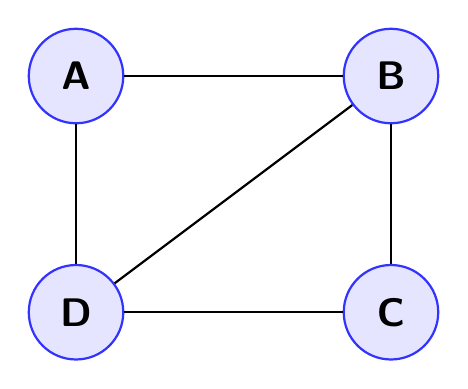
\begin{tikzpicture}[
    auto, 
    node distance=3cm, 
    thick,
    main node/.style={circle, fill=blue!10, draw=blue!80, minimum size=1.2cm, font=\sffamily\Large\bfseries}
]
    % Nodes
    \node[main node] (A) at (0, 0) {A};
    \node[main node] (B) at (4, 0) {B};
    \node[main node] (C) at (4, -3) {C};
    \node[main node] (D) at (0, -3) {D};

    % Edges (Bridges)
    \draw (A) -- (B);
    \draw (A) -- (D);
    \draw (B) -- (C);
    \draw (B) -- (D);
    \draw (C) -- (D);
\end{tikzpicture}
\end{center}

\begin{enumerate}
    \item Count the total number of connections for each node. \\
    \textit{(A = \_\_\_\_, \quad B = \_\_\_\_, \quad C = \_\_\_\_, \quad D = \_\_\_\_)}
    \item How many nodes have an \textbf{odd} number of connections? 
    \item Based purely on Euler's rule, is it mathematically possible to walk through this city and cross every single bridge exactly once? (Yes or No)
\end{enumerate}

\vspace{0.8cm}

\textbf{Problem 1.2: Reading the Map (Directed \& Weighted Graphs)} \\
The graph below represents a transportation network between three cities. The arrows indicate which direction traffic can flow, and the \textbf{Weights} represent the travel time in hours.

\begin{center}
\begin{tikzpicture}[
    ->, >=stealth, auto, node distance=3cm, thick,
    city node/.style={circle, fill=green!10, draw=green!60!black, minimum size=1.2cm, font=\sffamily\bfseries}
]
    % Nodes
    \node[city node] (City1) at (0, 0) {City 1};
    \node[city node] (City2) at (5, 0) {City 2};
    \node[city node] (City3) at (2.5, -3) {City 3};

    % Edges with weights
    \path[every node/.style={font=\sffamily\small, background color=white}]
        (City1) edge [bend left=15] node [above] {2 hrs} (City2)
        (City2) edge [bend left=15] node [below] {3 hrs} (City1)
        (City1) edge node [left] {4 hrs} (City3)
        (City3) edge node [right] {1 hr} (City2);
\end{tikzpicture}
\end{center}

\begin{enumerate}
    \item Is this graph \textbf{Directed} or \textbf{Undirected}? How do you know?
    \item If you are in City 3, can you travel directly to City 1? Why or why not?
    \item It takes 2 hours to get from City 1 to City 2. Why might the return trip (City 2 to City 1) have a different weight (3 hours)? Give a real-world example of why this might happen.
\end{enumerate}

% ----- Module 2 -----
\moduleheader{Module 2: Navigating the Network}

\textbf{Problem 2.1: The House Graph (Walks, Paths, \& Cycles)} \\
Below is a simple undirected graph shaped like a house. In the notebook, you learned the strict rules for how we move through a network. As a reminder: a \textbf{Walk} is any sequence of movements, a \textbf{Path} can never visit the same node twice, and a \textbf{Cycle} is a closed loop.

\begin{center}
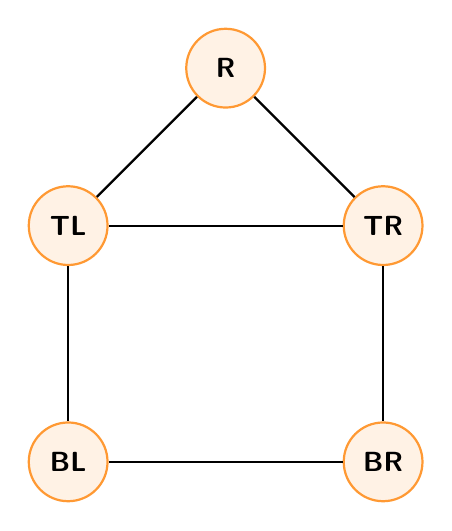
\begin{tikzpicture}[
    auto, 
    node distance=2.5cm, 
    thick,
    main node/.style={circle, fill=orange!10, draw=orange!80, minimum size=1cm, font=\sffamily\bfseries}
]
    % Nodes
    \node[main node] (Roof) at (2, 2) {R};
    \node[main node] (TL) at (0, 0) {TL};
    \node[main node] (TR) at (4, 0) {TR};
    \node[main node] (BL) at (0, -3) {BL};
    \node[main node] (BR) at (4, -3) {BR};

    % Edges
    \draw (Roof) -- (TL);
    \draw (Roof) -- (TR);
    \draw (TL) -- (TR);
    \draw (TL) -- (BL);
    \draw (TR) -- (BR);
    \draw (BL) -- (BR);
\end{tikzpicture}
\end{center}

\begin{enumerate}
    \item List the nodes in a valid \textbf{Cycle} of length 3 (a triangle).
    \item A student traces the following route: \textbf{R $\rightarrow$ TL $\rightarrow$ TR $\rightarrow$ R $\rightarrow$ BR}. \\
    Is this route a \textbf{Path}? Why or why not?
    \item Trace a valid \textbf{Path} that starts at the Roof (R) and visits \textit{every single other node} exactly once before stopping.
\end{enumerate}

\vspace{0.8cm}

\textbf{Problem 2.2: The Rumor Mill (Degrees \& Hops)} \\
The graph below represents a high school social network of 8 students. A line between two students means they text each other. We want to find out who the most popular student is, and how fast a rumor can spread.

\begin{center}
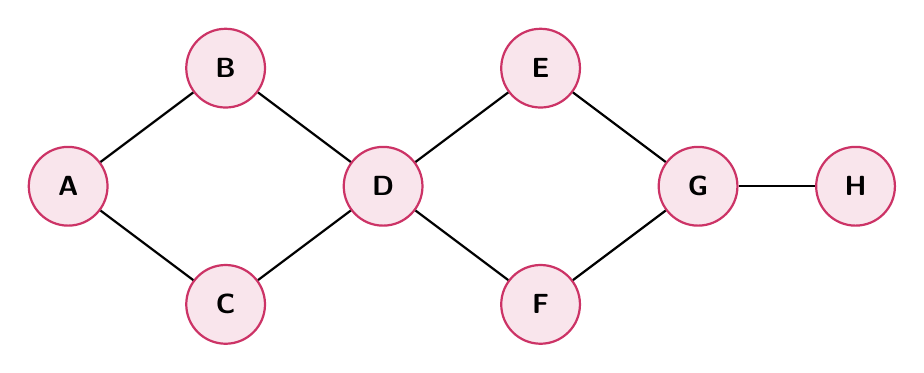
\begin{tikzpicture}[
    auto, 
    node distance=2cm, 
    thick,
    student node/.style={circle, fill=purple!10, draw=purple!80, minimum size=1cm, font=\sffamily\bfseries}
]
    % Nodes
    \node[student node] (A) at (0, 0) {A};
    \node[student node] (B) at (2, 1.5) {B};
    \node[student node] (C) at (2, -1.5) {C};
    \node[student node] (D) at (4, 0) {D};
    \node[student node] (E) at (6, 1.5) {E};
    \node[student node] (F) at (6, -1.5) {F};
    \node[student node] (G) at (8, 0) {G};
    \node[student node] (H) at (10, 0) {H};

    % Edges
    \draw (A) -- (B);
    \draw (A) -- (C);
    \draw (B) -- (D);
    \draw (C) -- (D);
    \draw (D) -- (E);
    \draw (D) -- (F);
    \draw (E) -- (G);
    \draw (F) -- (G);
    \draw (G) -- (H);
\end{tikzpicture}
\end{center}

\begin{enumerate}
    \item The \textbf{Degree} of a node is its number of direct connections. Which student has the highest degree (the "Hub"), and what is their degree?
    \item Student A starts a rumor. What is the shortest distance, measured in \textbf{Hops}, for the rumor to reach Student H? Write out the shortest path.
    \item Imagine Student D's phone breaks, removing them (and all their edges) from the network entirely. Can a rumor from Student A still reach Student H? If yes, how many hops does it take now? If no, explain why.
\end{enumerate}

% ----- Module 3 -----
\moduleheader{Module 3: Topologies (The Zoo of Shapes)}

\textbf{Problem 3.1: The Power Grid (Network Robustness)} \\
Below are two different designs for a city's power grid. Graph 1 uses a \textbf{Star} topology, while Graph 2 uses a \textbf{Ring} (Cycle) topology. In network science, we care deeply about "Robustness"—how well a network survives when a node breaks down.

\begin{center}
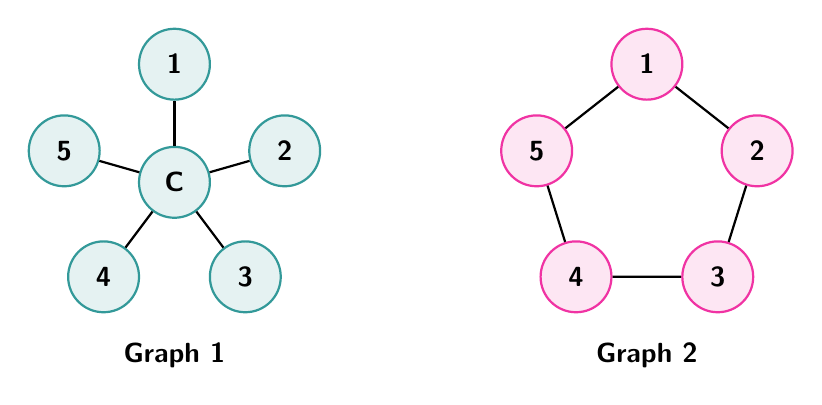
\begin{tikzpicture}[
    auto, 
    thick,
    star node/.style={circle, fill=teal!10, draw=teal!80, minimum size=0.9cm, font=\sffamily\bfseries},
    ring node/.style={circle, fill=magenta!10, draw=magenta!80, minimum size=0.9cm, font=\sffamily\bfseries}
]
    % --- Graph 1: Star ---
    \node[star node] (Center) at (0, 0) {C};
    \node[star node] (S1) at (0, 1.5) {1};
    \node[star node] (S2) at (1.4, 0.4) {2};
    \node[star node] (S3) at (0.9, -1.2) {3};
    \node[star node] (S4) at (-0.9, -1.2) {4};
    \node[star node] (S5) at (-1.4, 0.4) {5};
    
    \draw (Center) -- (S1);
    \draw (Center) -- (S2);
    \draw (Center) -- (S3);
    \draw (Center) -- (S4);
    \draw (Center) -- (S5);
    
    \node[font=\sffamily\bfseries] at (0, -2.2) {Graph 1};

    % --- Graph 2: Ring ---
    \begin{scope}[shift={(6, 0)}]
        \node[ring node] (R1) at (0, 1.5) {1};
        \node[ring node] (R2) at (1.4, 0.4) {2};
        \node[ring node] (R3) at (0.9, -1.2) {3};
        \node[ring node] (R4) at (-0.9, -1.2) {4};
        \node[ring node] (R5) at (-1.4, 0.4) {5};
        
        \draw (R1) -- (R2) -- (R3) -- (R4) -- (R5) -- (R1);
        \node[font=\sffamily\bfseries] at (0, -2.2) {Graph 2};
    \end{scope}
\end{tikzpicture}
\end{center}

\begin{enumerate}
    \item Imagine a storm destroys Node C in Graph 1. How many separate, isolated pieces does the network break into?
    \item Imagine a storm destroys Node 1 in Graph 2. Can Node 2 still communicate with Node 5? If yes, what is the new shortest path (in hops) between them?
    \item Based on your answers, which topology is better for a hospital's backup generators, and which is better for a fast, centralized computer server?
\end{enumerate}

\vspace{0.6cm}

\textbf{Problem 3.2: The Recommendation Algorithm (Bipartite Graphs)} \\
A \textbf{Bipartite Graph} splits nodes into two distinct groups (e.g., Users and Movies) where edges can \textit{only} connect a node from Group A to a node in Group B. 

\begin{center}
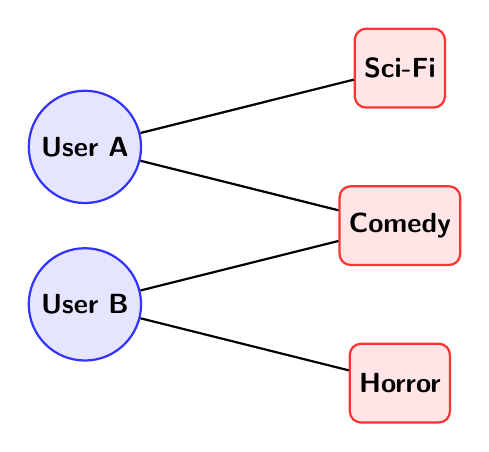
\begin{tikzpicture}[
    auto, 
    thick,
    user node/.style={circle, fill=blue!10, draw=blue!80, minimum size=1cm, font=\sffamily\bfseries},
    movie node/.style={rectangle, rounded corners, fill=red!10, draw=red!80, minimum size=1cm, font=\sffamily\bfseries}
]
    % Users
    \node[user node] (U1) at (0, 1) {User A};
    \node[user node] (U2) at (0, -1) {User B};
    
    % Movies
    \node[movie node] (M1) at (4, 2) {Sci-Fi};
    \node[movie node] (M2) at (4, 0) {Comedy};
    \node[movie node] (M3) at (4, -2) {Horror};

    % Edges
    \draw (U1) -- (M1);
    \draw (U1) -- (M2);
    \draw (U2) -- (M2);
    \draw (U2) -- (M3);
\end{tikzpicture}
\end{center}

\begin{enumerate}
    \item A programmer accidentally adds an edge directly between \textbf{User A} and \textbf{User B}. Why does this instantly break the mathematical definition of a Bipartite Graph?
\end{enumerate}

\vspace{0.6cm}

\textbf{Problem 3.3: The Microchip Puzzle (Planar Graphs)} \\
A graph is \textbf{Planar} if it can be drawn on a flat piece of paper without \textit{any} of its edges crossing over one another. Below is a Complete Graph of 4 nodes ($K_4$). Right now, the diagonal lines cross in the center.

\begin{center}
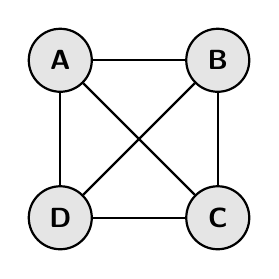
\begin{tikzpicture}[
    auto, 
    thick,
    main node/.style={circle, fill=gray!20, draw=black, minimum size=0.8cm, font=\sffamily\bfseries}
]
    \node[main node] (A) at (0, 2) {A};
    \node[main node] (B) at (2, 2) {B};
    \node[main node] (C) at (2, 0) {C};
    \node[main node] (D) at (0, 0) {D};

    \draw (A) -- (B);
    \draw (B) -- (C);
    \draw (C) -- (D);
    \draw (D) -- (A);
    \draw (A) -- (C); % Diagonal 1
    \draw (B) -- (D); % Diagonal 2
\end{tikzpicture}
\end{center}

\begin{enumerate}
    \item Prove that this graph is actually Planar! In the empty space below, redraw the 4 nodes and all 6 edges, but move one of the diagonal lines so that \textbf{no lines cross}. \textit{(Hint: You are allowed to draw lines outside the square!)}
\end{enumerate}
\vspace{3cm}

% ----- Module 4 -----
\moduleheader{Module 4: Applied Graph Theory (The Real World)}

\textbf{Problem 4.1: The Influencer Target (Degree Centrality)} \\
You are running a marketing campaign for a new app with a very limited budget. You only have enough money to sponsor \textit{one} user in the network below. In the notebook, you learned that "Degree Centrality" helps us find the "Hubs."

\begin{center}
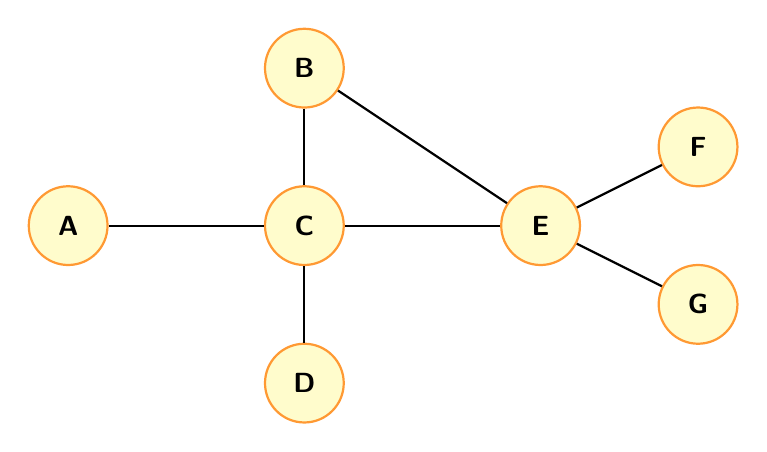
\begin{tikzpicture}[
    auto, 
    thick,
    user node/.style={circle, fill=yellow!20, draw=orange!80, minimum size=1cm, font=\sffamily\bfseries}
]
    % Nodes
    \node[user node] (A) at (0, 0) {A};
    \node[user node] (B) at (3, 2) {B};
    \node[user node] (C) at (3, 0) {C};
    \node[user node] (D) at (3, -2) {D};
    \node[user node] (E) at (6, 0) {E};
    \node[user node] (F) at (8, 1) {F};
    \node[user node] (G) at (8, -1) {G};

    % Edges
    \draw (A) -- (C);
    \draw (B) -- (C);
    \draw (D) -- (C);
    \draw (C) -- (E);
    \draw (E) -- (F);
    \draw (E) -- (G);
    \draw (B) -- (E); % Extra connection
\end{tikzpicture}
\end{center}

\begin{enumerate}
    \item What is the \textbf{Degree} of Node C? What is the \textbf{Degree} of Node E?
    \item If a rumor travels one edge (one hop) per day, and you sponsor Node F, how many days will it take for the rumor to reach Node A?
    \item Based purely on Degree Centrality, which node is the most powerful "Influencer" in this network, and why is sponsoring them the most efficient strategy?
\end{enumerate}

\vspace{0.6cm}

\end{enumerate}

\end{document}

